\chapter{Results}
\label{ch:results}

\section{Reactor Condition and Visual Observations}
\label{sec:reactor_condition}

The reactor was inoculated with anaerobic sludge and initially contained a murky, light brown suspension (\cref{fig:reactor_murky}). Within three days of operation, the colour changed to black (\cref{fig:reactor_black}), which is characteristic of active anaerobic digestion and is typically caused by the precipitation of metal sulphides, particularly iron sulphide, under reducing conditions. This visual change indicated the establishment of a suitable anaerobic environment and the onset of methanogenic activity.

\begin{figure}
    \centering
    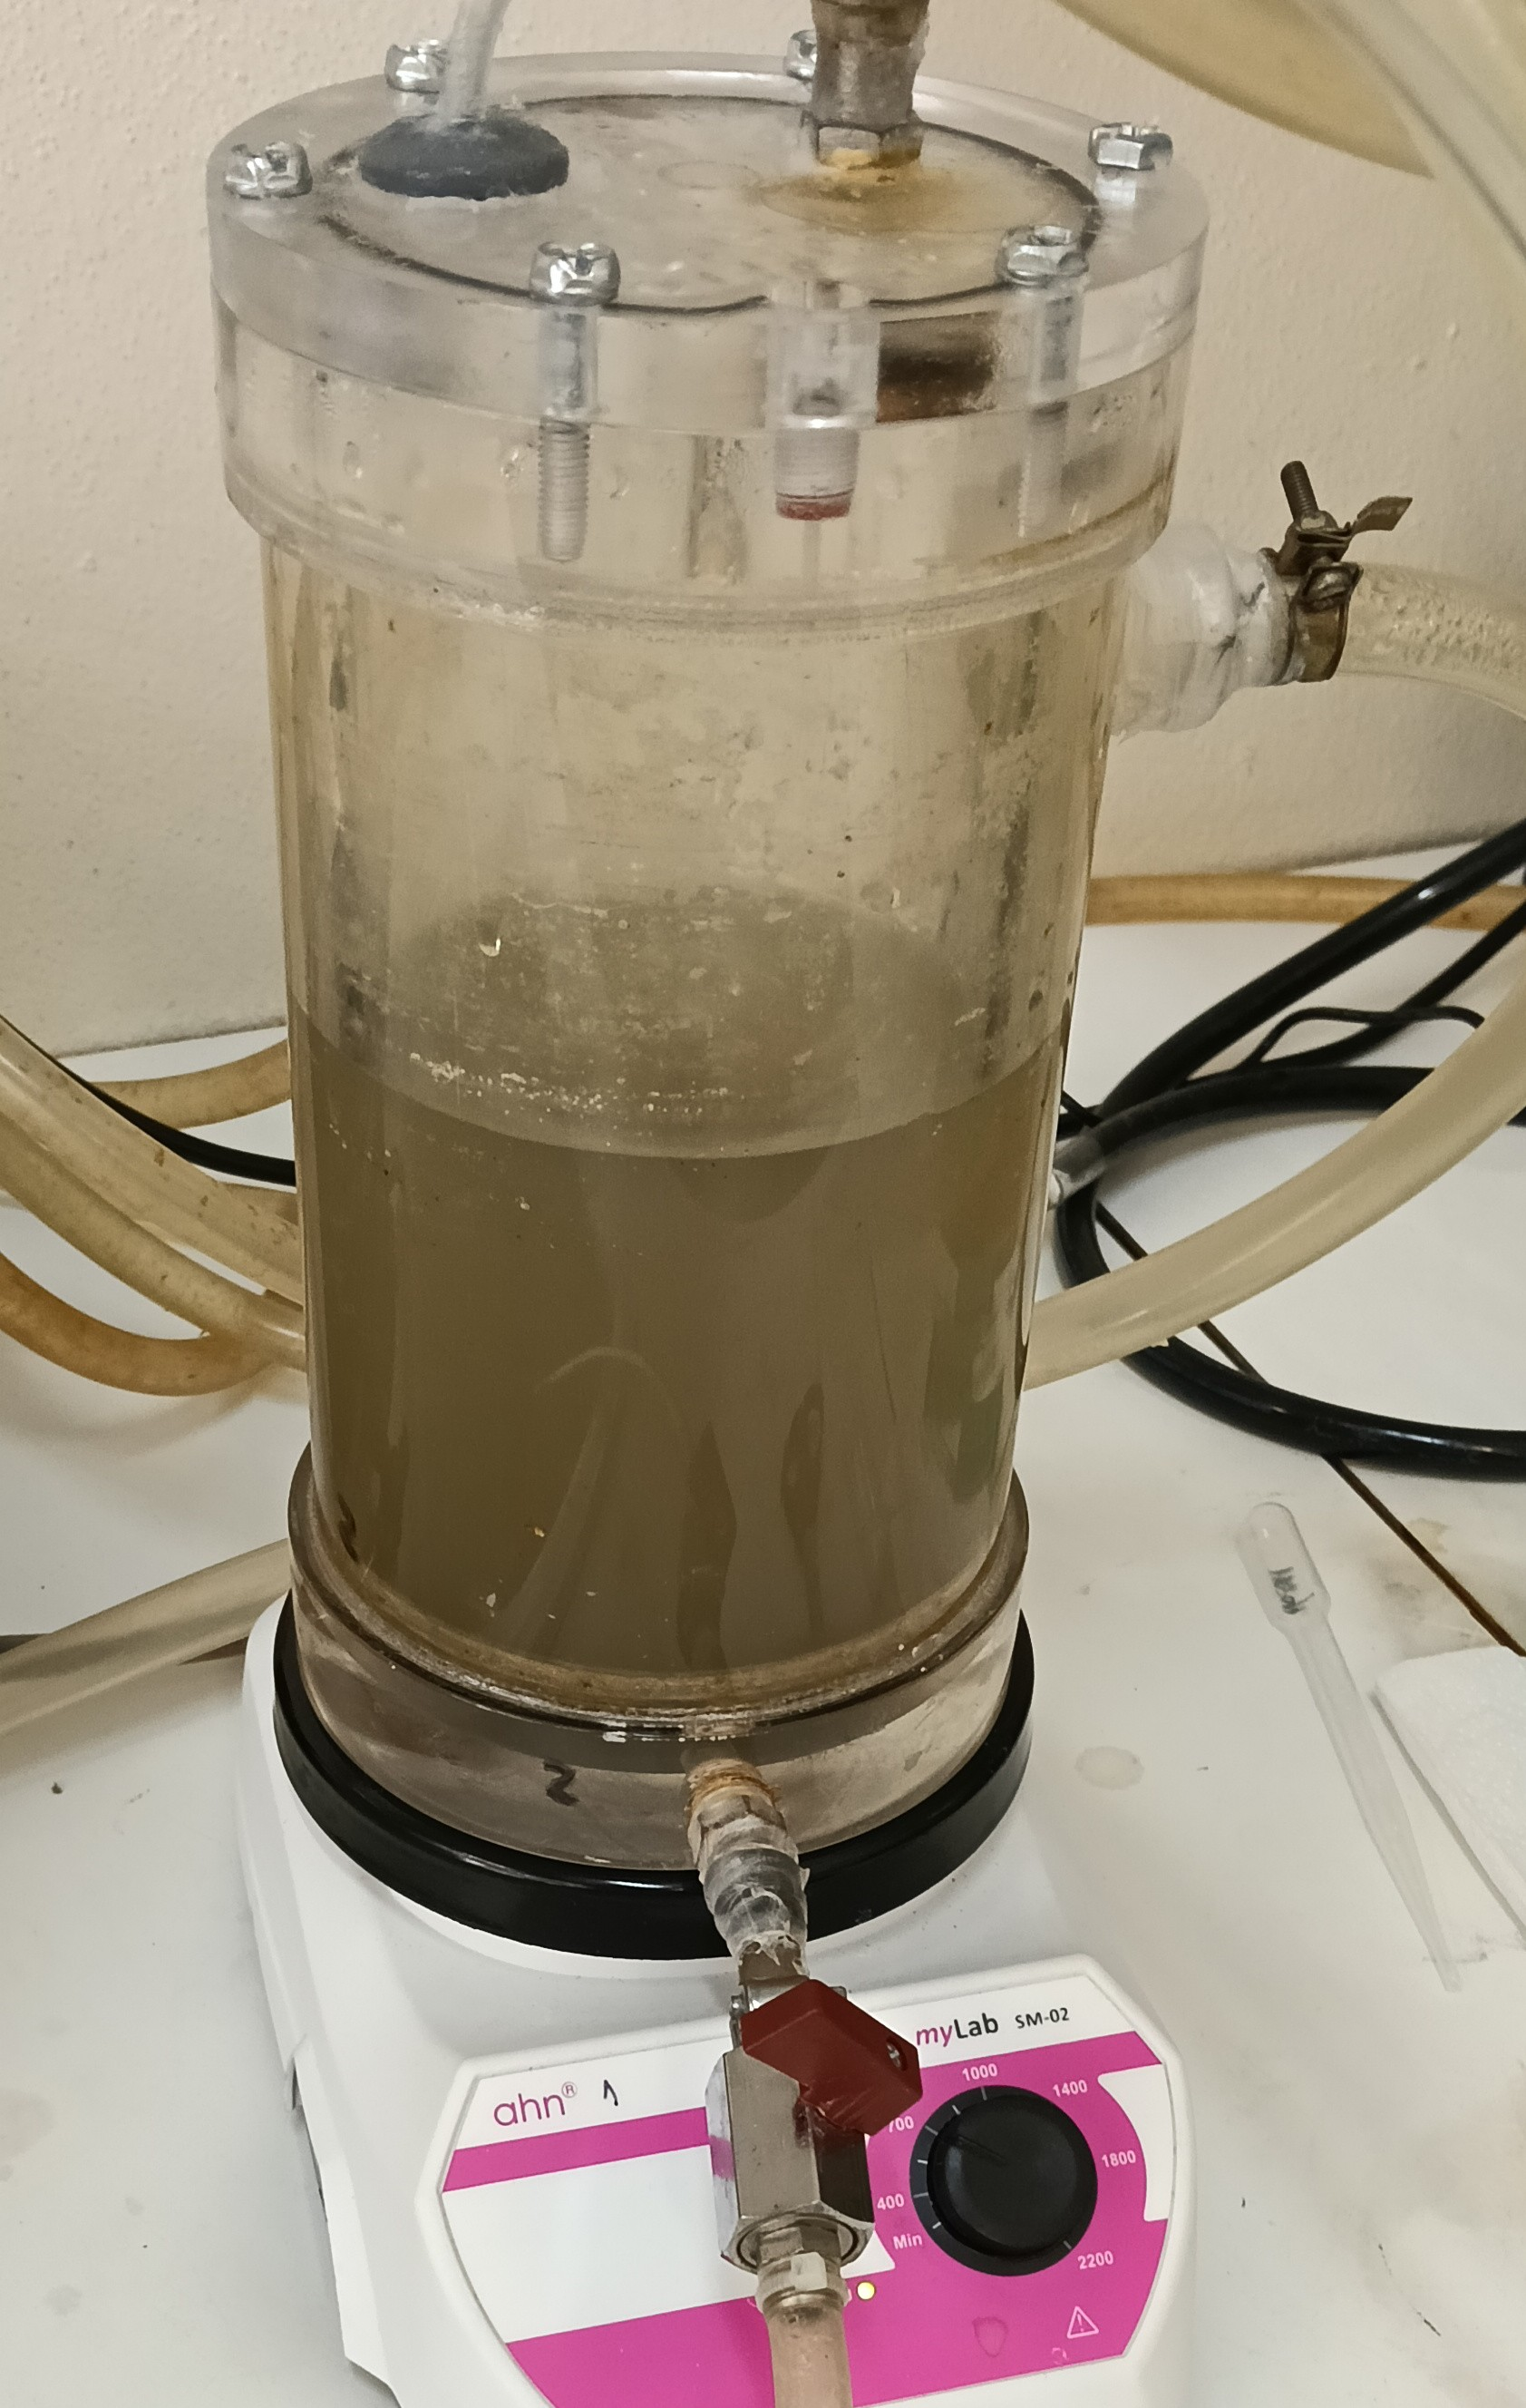
\includegraphics[width=0.4\textwidth]{assets/reator-19-5.jpg}
    \caption{Source: Author}
    \label{fig:reactor_murky}
\end{figure}

\begin{figure}
    \centering
    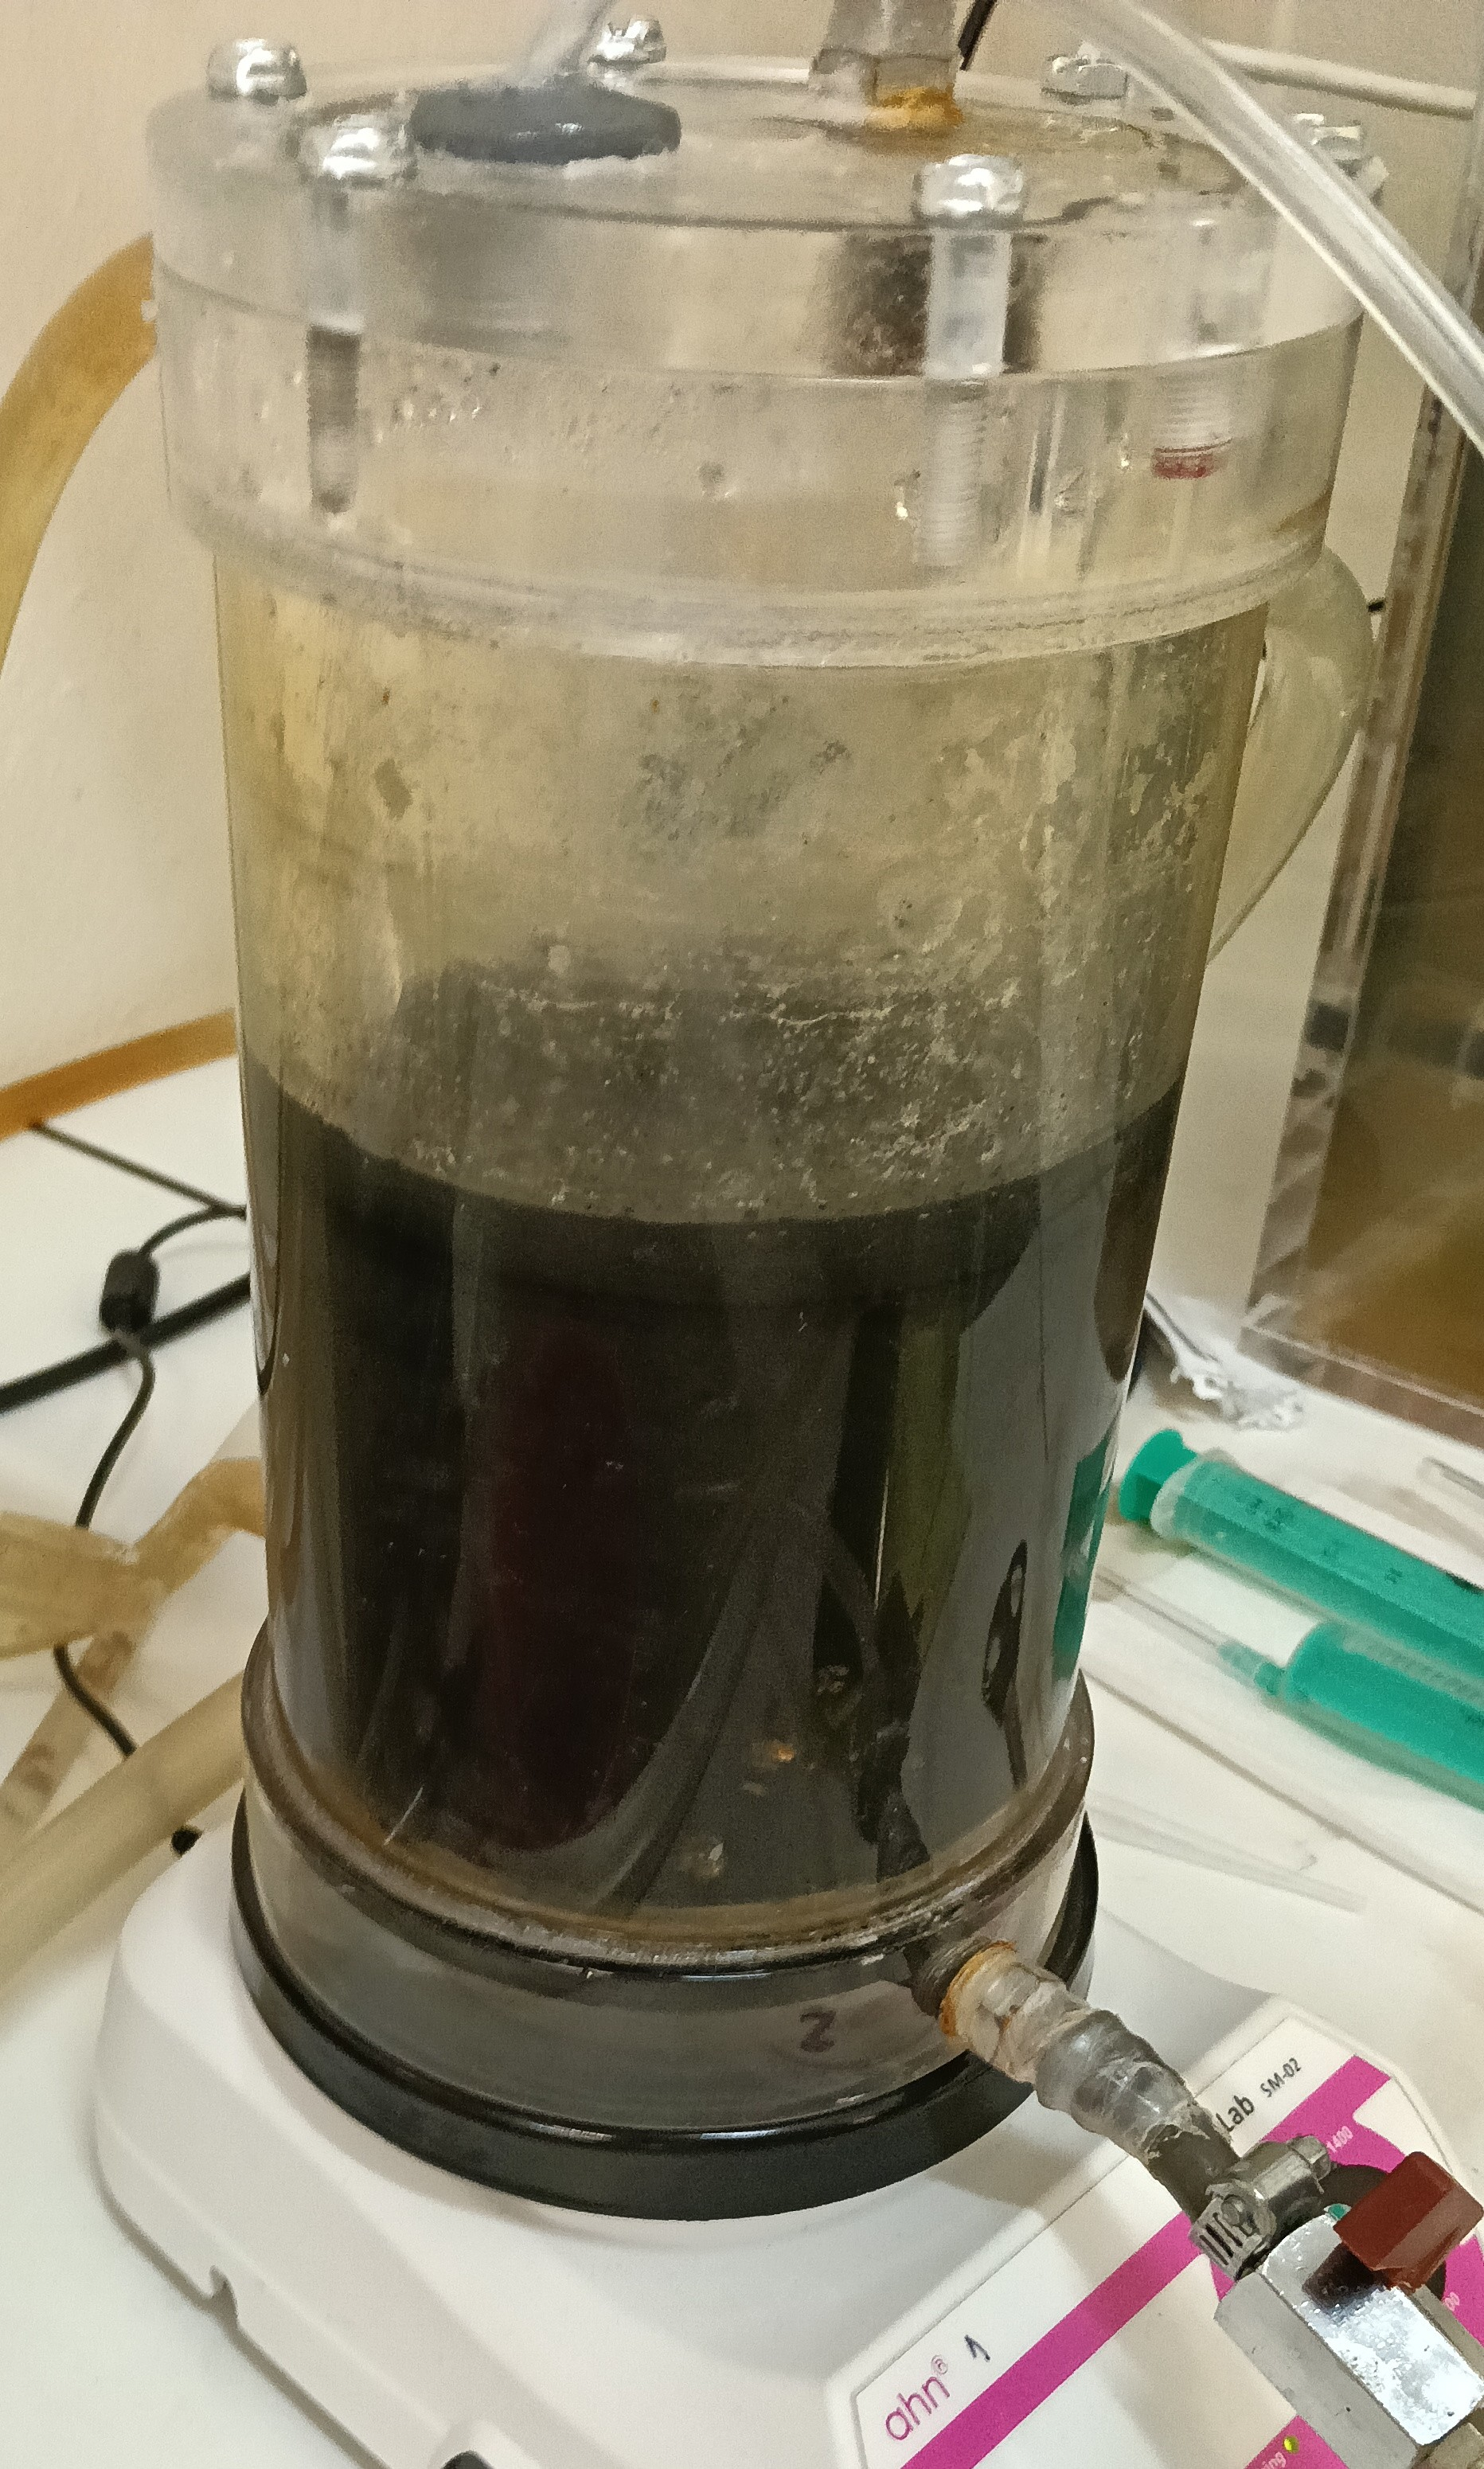
\includegraphics[width=0.4\textwidth]{assets/reator-22-5.jpg}
    \caption{Source: Author}
    \label{fig:reactor_black}
\end{figure}

At the end of the experimental period, after approximately two weeks of unattended operation, four discrete masses resembling fungal colonies were observed on the internal surfaces of the reactor during cleaning (\cref{fig:masses-dry,fig:masses-wet}). The origin of these growths is uncertain, but they may have been introduced via the food waste feed or during periods when the feeding tube was opened for repairs (e.g. leaks) and when cahnging the feed that the tube had to be cleaned. The presence of such organisms could have competed with the anaerobic microbial community for substrate, potentially affecting biogas production in the later stages of the experiment.

\begin{figure}
    \centering
    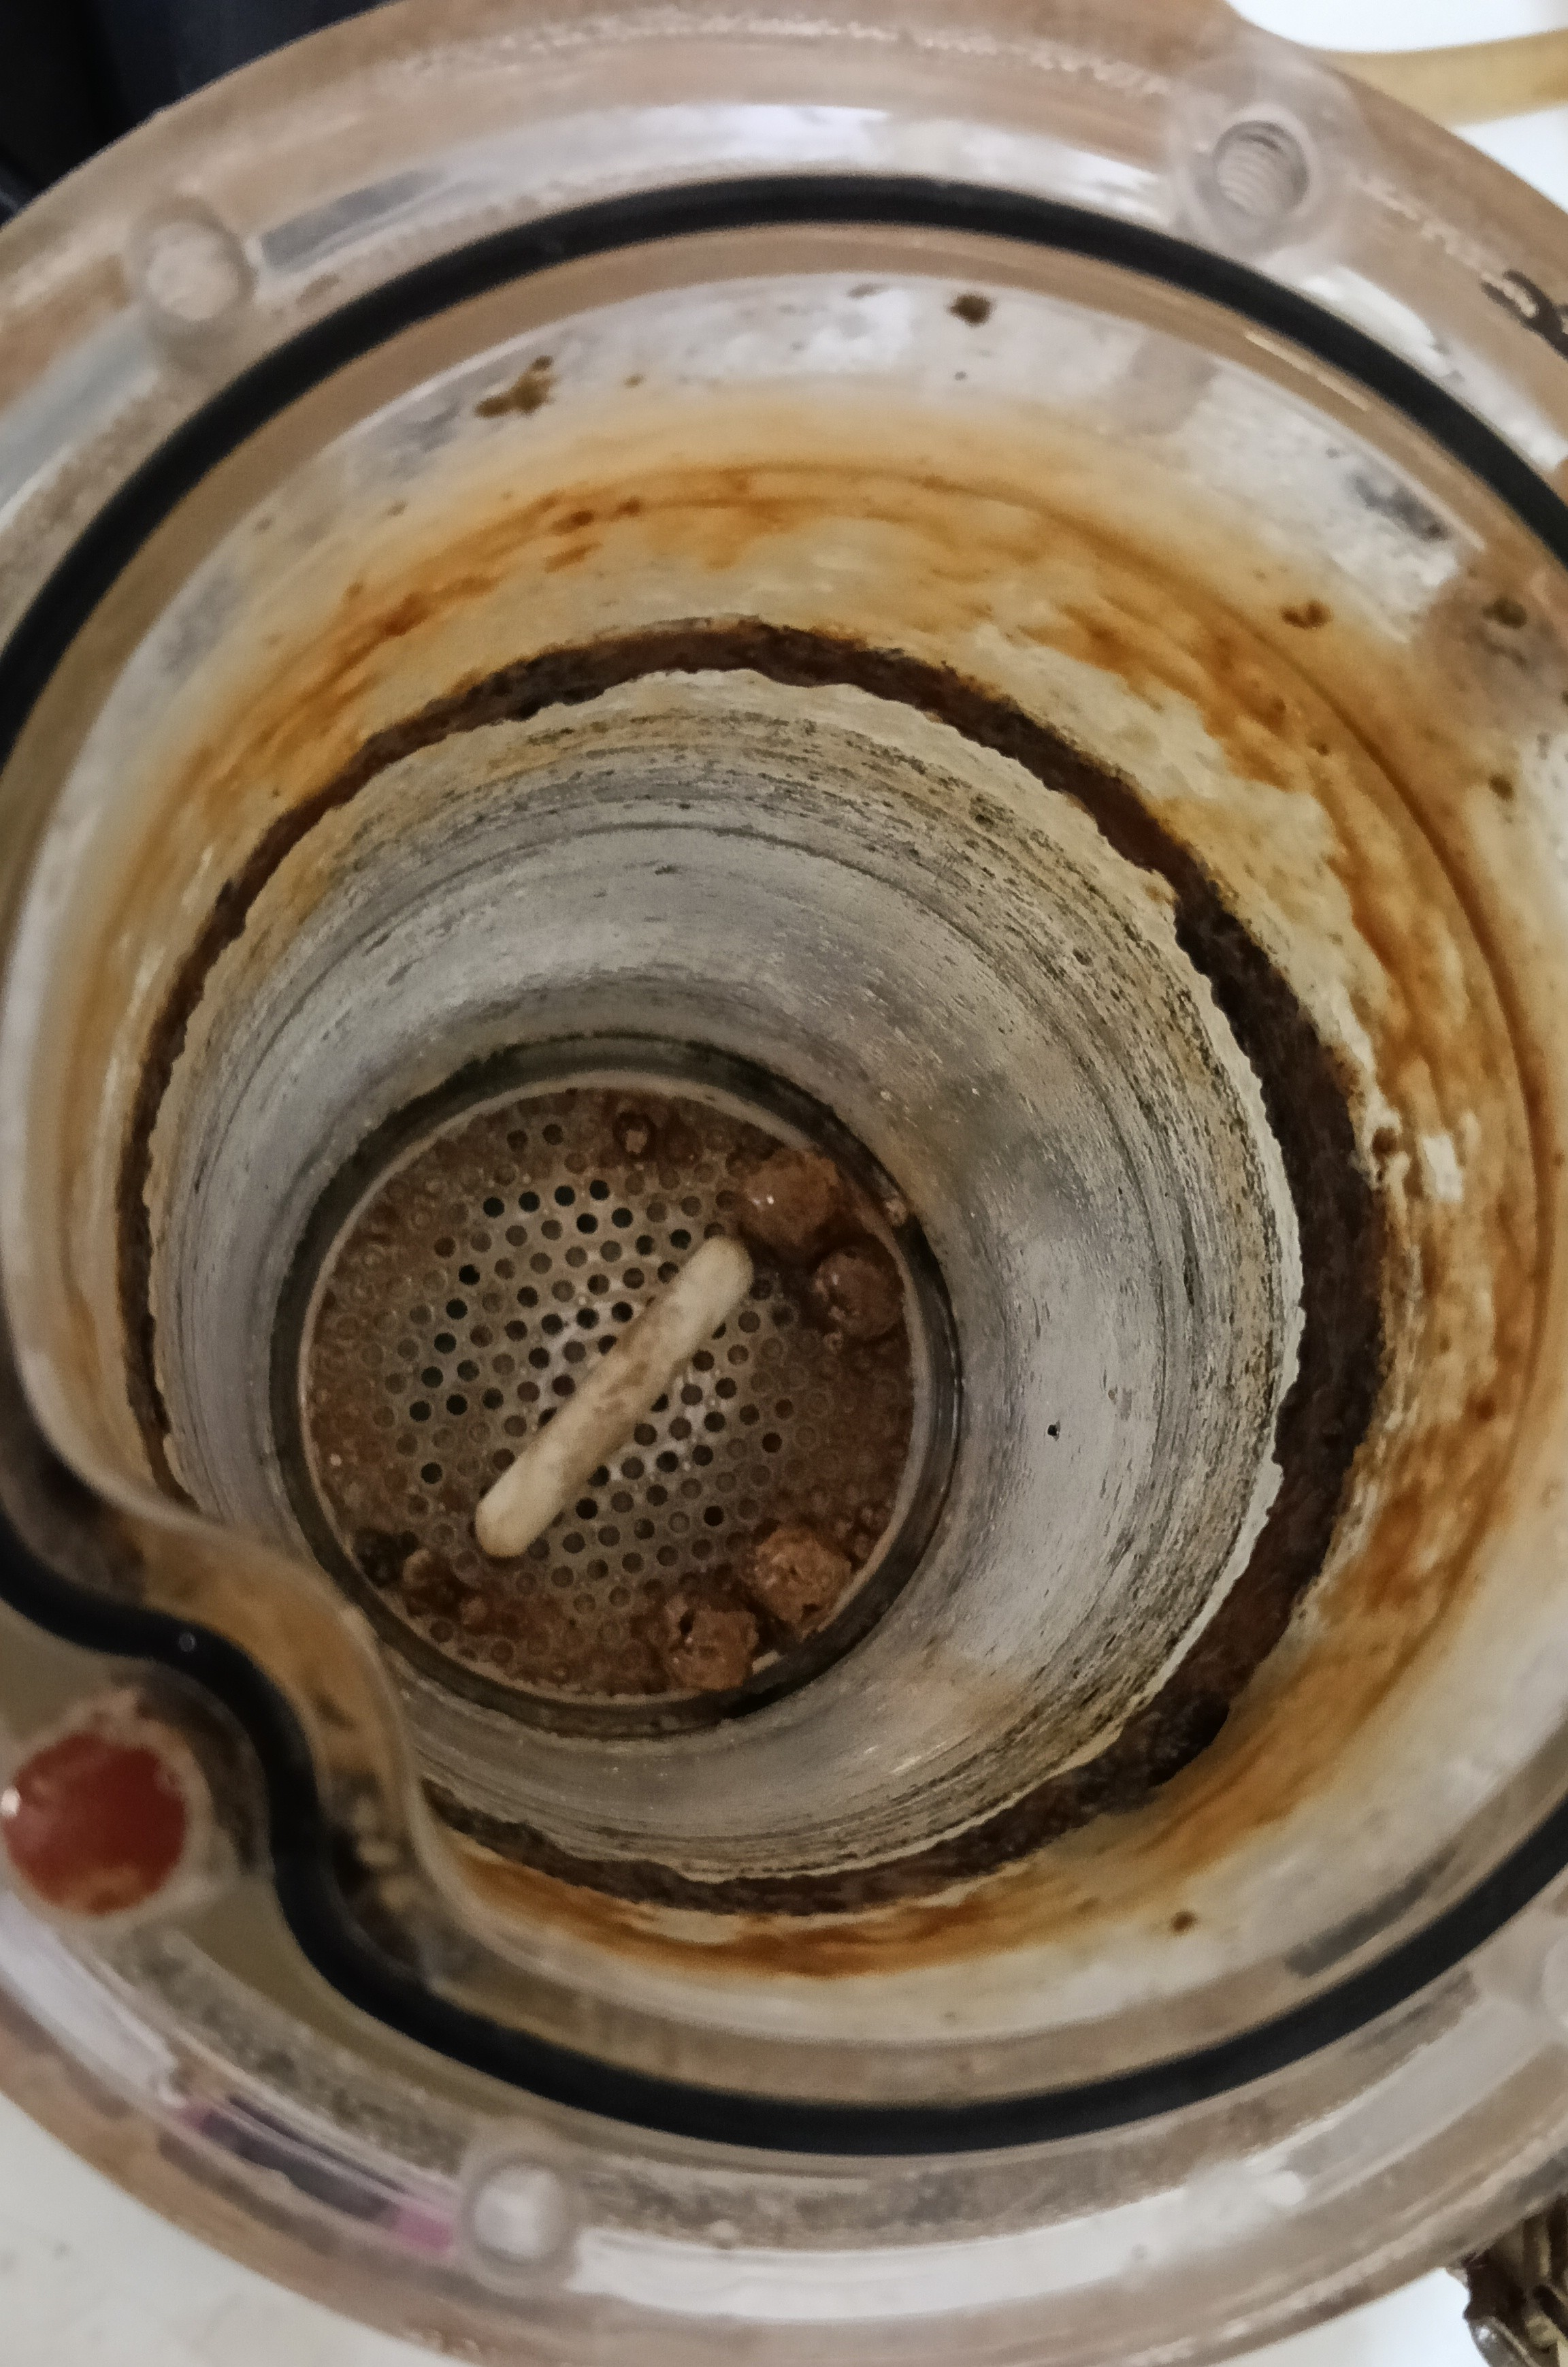
\includegraphics[width=0.4\textwidth]{assets/reator-limp-seco-24-8.jpg}
    \caption{Source: Author}
    \label{fig:masses-dry}
\end{figure}

\begin{figure}
    \centering
    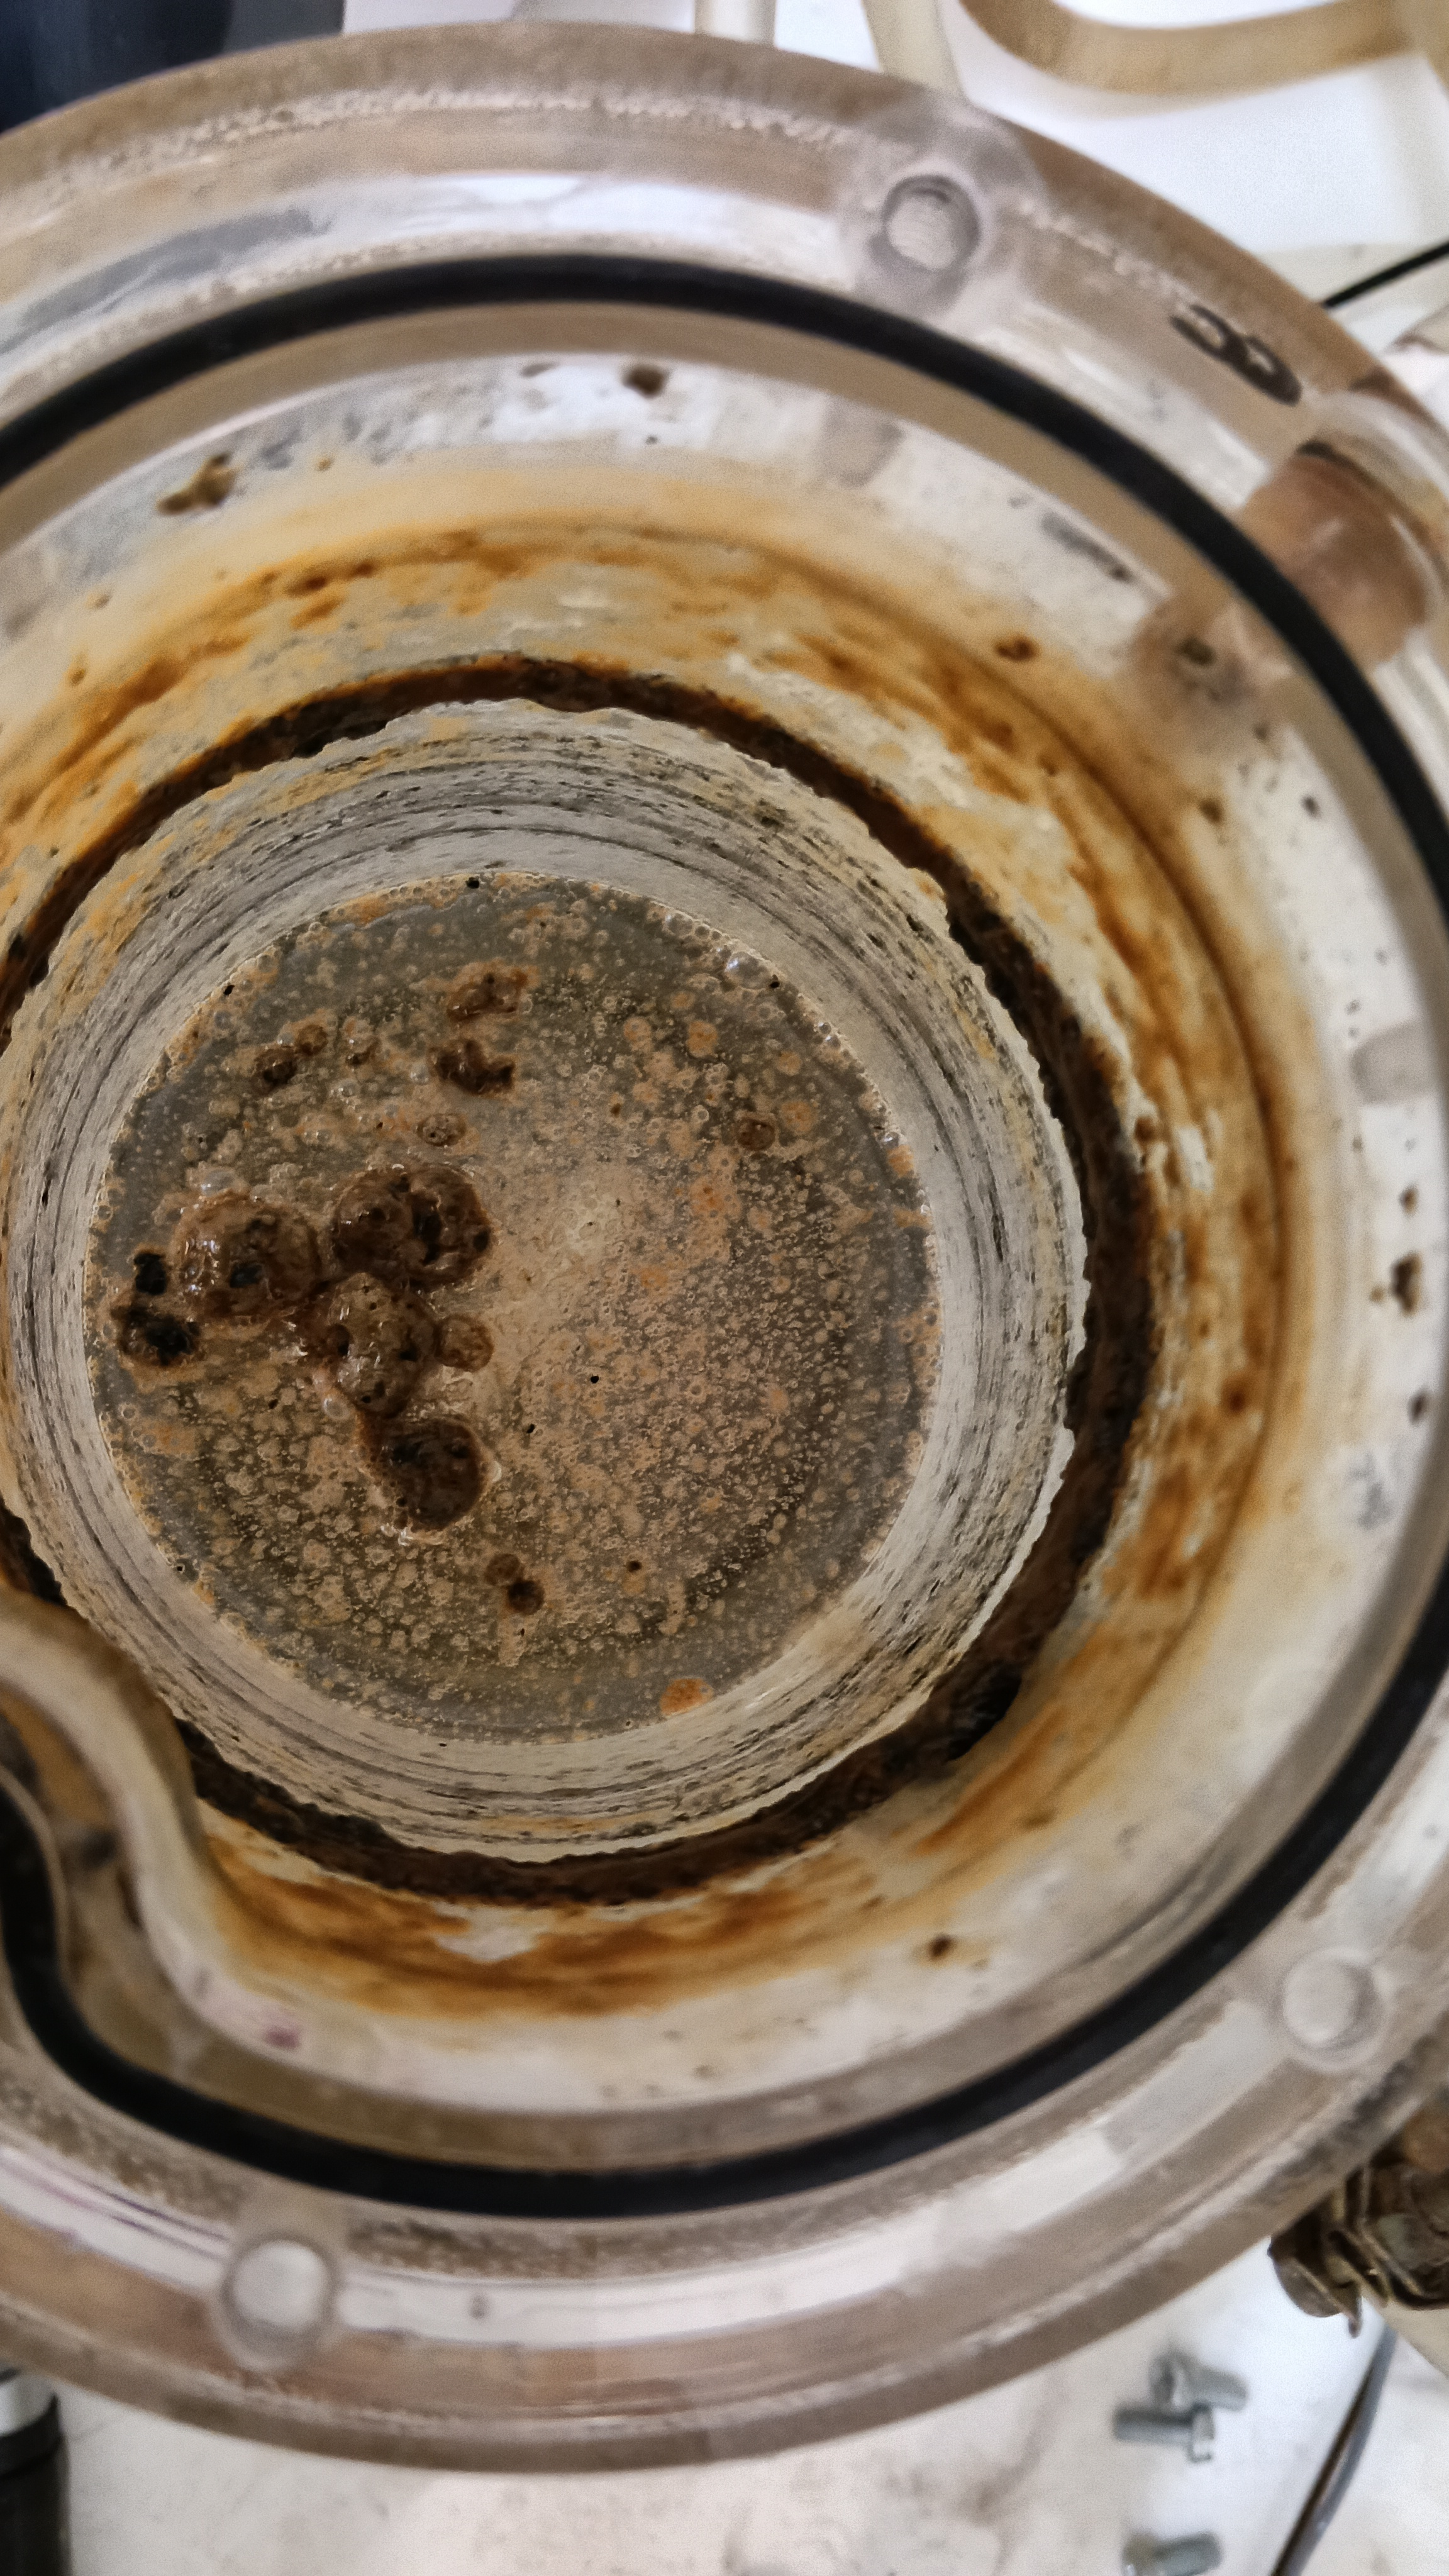
\includegraphics[width=0.4\textwidth]{assets/reator-limp-agua-24-8.jpg}
    \caption{Source: Author}
    \label{fig:masses-wet}
\end{figure}

\section{Biogas Production}
\label{sec:biogas_production}

Biogas production was monitored continuously using AMPTS II, which recorded both the cumulative volume of methane produced and the instantaneous flow rate. The entire experimental period is summarised in \cref{graph:total-accumulation,graph:total-flow}. To facilitate interpretation, the data have been divided into four distinct phases based on the feeding regime: (i) an adaptation phase~\ref{subsec:adaptation_phase}, (ii) co-digestion of food waste and glycerol~\ref{subsec:codigestion_phase}, (iii) glycerol only feeding~\ref{subsec:glycerol_phase}, and (iv) a post-feeding period~\ref{subsec:post_feeding}.

\begin{graph}
    \centering
    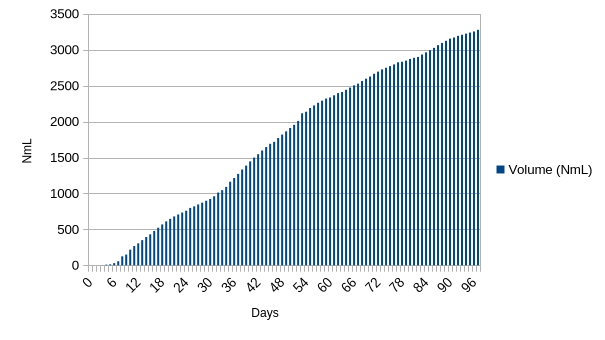
\includegraphics[width=\textwidth]{assets/graphs/total-accumulation.png}
    \caption{Source: Author}
    \label{graph:total-accumulation}
\end{graph}

\begin{graph}
    \centering
    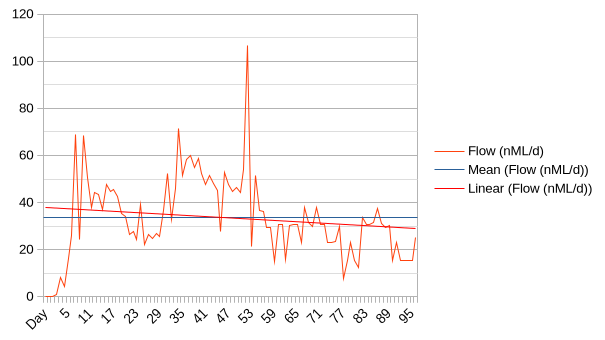
\includegraphics[width=\textwidth]{assets/graphs/total-flow.png}
    \caption{Source: Author}
    \label{graph:total-flow}
\end{graph}

\subsection{Overall Production}
\label{subsec:overall_production}

The cumulative methane production over the whole experiment (\cref{graph:total-accumulation}) shows a continuous increase, indicating that the reactor maintained methanogenic activity throughout the monitored period. The total flow profile (\cref{graph:total-flow}) exhibits distinct peaks corresponding to daily feeding events, with variations in amplitude reflecting the different substrate compositions and organic loading rates applied during each phase. And a outlier peak at day 53, that was when the feed was changed from a mixture of food waste and crude glycerol, to only crude glycerol, and due to some complications, there was that anomaly.

\subsection{Adaptation Phase}
\label{subsec:adaptation_phase}

During the initial adaptation phase, biogas production was low (\cref{graph:pre-accumulation,graph:pre-flow}). This lag period is normal for anaerobic reactors as the microbial community adjusts to the new substrate and operating conditions. The small but measurable methane flow confirmed that the viability of the inoculum, and the gradual increase in flow suggested the onset of exponential growth of the microorganisms.

\begin{graph}
    \centering
    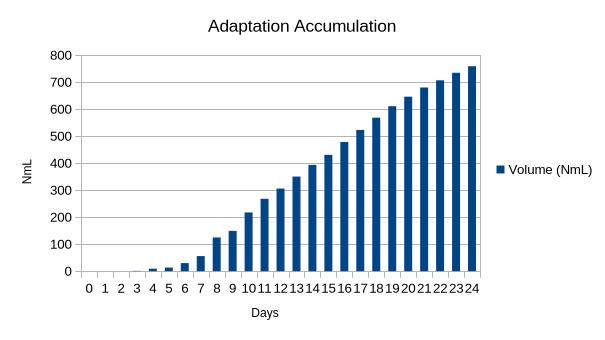
\includegraphics[width=\textwidth]{assets/graphs/pre-accumulation.png}
    \caption{Source: Author}
    \label{graph:pre-accumulation}
\end{graph}

\begin{graph}
    \centering
    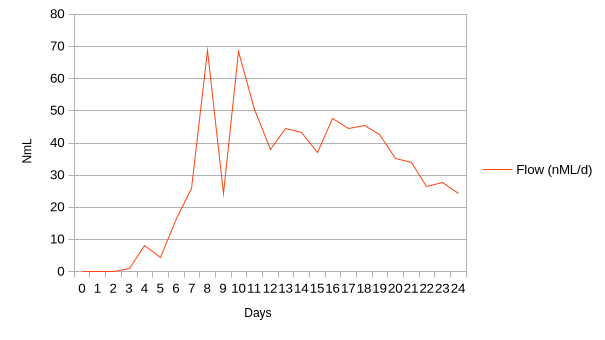
\includegraphics[width=\textwidth]{assets/graphs/pre-flow.png}
    \caption{Source: Author}
    \label{graph:pre-flow}
\end{graph}

\subsection{Co-digestion of Food Waste and Glycerol}
\label{subsec:codigestion_phase}

The reactor was fed with a mixture of food waste and crude glycerol with a higher concentration, a marked increase in biogas production was observed (\cref{graph:ra-accumulation,graph:ra-flow}). The cumulative methane volume rose steeply, and the flow rate showed pronounced spikes immediately after each feeding event (\cref{graph:ra-flow-30}). These spikes are typical of readily degradable substrates, which are quickly hydrolysed and converted to volatile fatty acids and subsequently to methane. The average flow rate during this phase was higher than in any other phase, indicating that the co-digestion of food waste and glycerol provided a balanced nutrient supply and avoided the inhibition often associated with high glycerol concentrations alone.

\begin{graph}
    \centering
    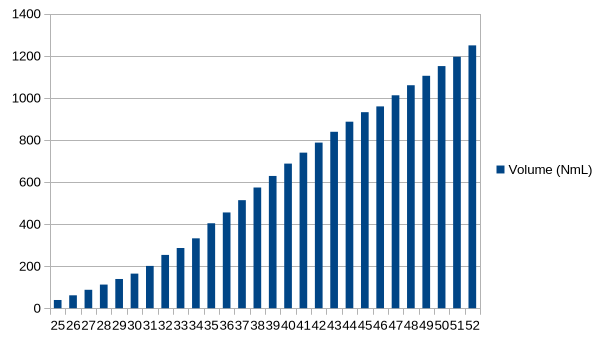
\includegraphics[width=\textwidth]{assets/graphs/ra-accumulation.png}
    \caption{Source: Author}
    \label{graph:ra-accumulation}
\end{graph}

\begin{graph}
    \centering
    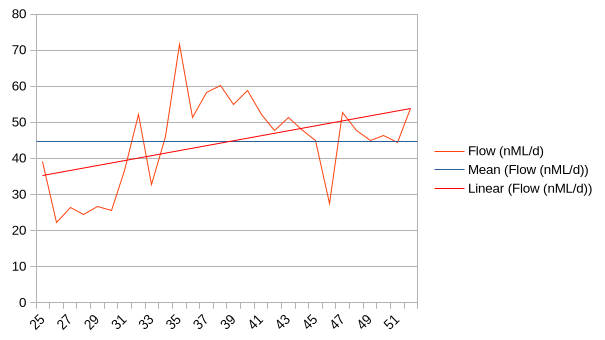
\includegraphics[width=\textwidth]{assets/graphs/ra-flow.png}
    \caption{Source: Author}
    \label{graph:ra-flow}
\end{graph}

\begin{graph}
    \centering
    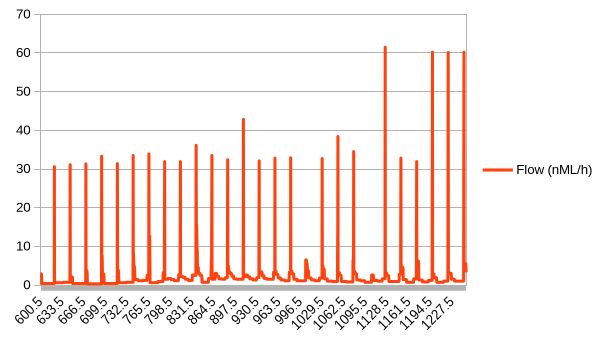
\includegraphics[width=\textwidth]{assets/graphs/ra-flow-30.png}
    \caption{Source: Author}
    \label{graph:ra-flow-30}
\end{graph}

\subsection{Glycerol only Feeding Period}
\label{subsec:glycerol_phase}

When the feed was changed to crude glycerol alone, biogas production decreased noticeably (\cref{graph:gl-accumulation,graph:gl-flow}). Although spikes in flow were still observed after feeding (\cref{graph:gl-flow-30}), their magnitude was bigger than during the co-digestion phase, and the cumulative methane volume plateaued more quickly. Several factors may explain this lower performance:
\begin{itemize}
    \item The glycerol could have been transformed to fast or too slow, to maintaing a concentration of intermediate products.
    \item The hydraulic retention time of 30 days may have been insufficient to wash out inhibitory by‑products or to maintain a stable population of glycerol‑fermenting bacteria.
    \item The appearance of fungal masses towards the end of this phase could have further stressed the anaerobic community by competing for substrate or introducing toxic metabolites.
\end{itemize}

\begin{graph}
    \centering
    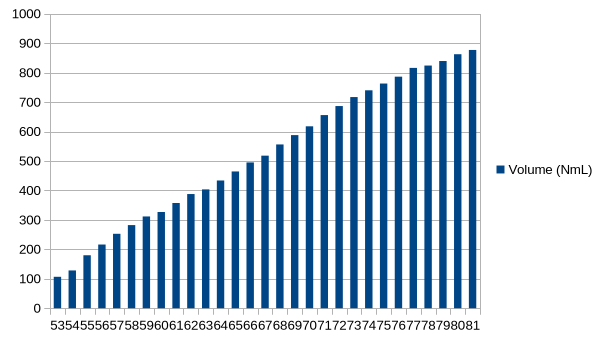
\includegraphics[width=\textwidth]{assets/graphs/gl-accumulation.png}
    \caption{Source: Author}
    \label{graph:gl-accumulation}
\end{graph}

\begin{graph}
    \centering
    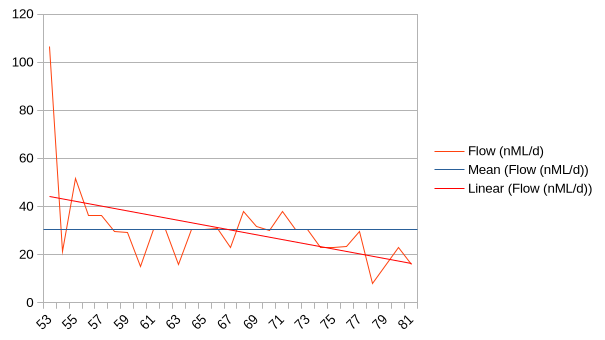
\includegraphics[width=\textwidth]{assets/graphs/gl-flow.png}
    \caption{Source: Author}
    \label{graph:gl-flow}
\end{graph}

\begin{graph}
    \centering
    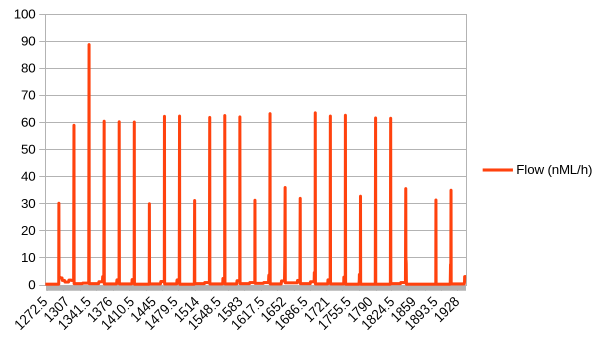
\includegraphics[width=\textwidth]{assets/graphs/gl-flow-30.png}
    \caption{Source: Author}
    \label{graph:gl-flow-30}
\end{graph}

\subsection{Post-feeding Period}
\label{subsec:post_feeding}

During the final two weeks, no fresh substrate was added to the reactor, it just had some residual substrate from the glycerol only phase for a week. Nevertheless, a small residual biogas production was recorded (\cref{graph:extra-accumulation,graph:extra-flow}). This production can be attributed to the slow degradation of accumulated organic matter and microbial decay products. The flow rate declined gradually, confirming that the reactor was no longer being actively fed and that the remaining substrate was limited.

\begin{graph}
    \centering
    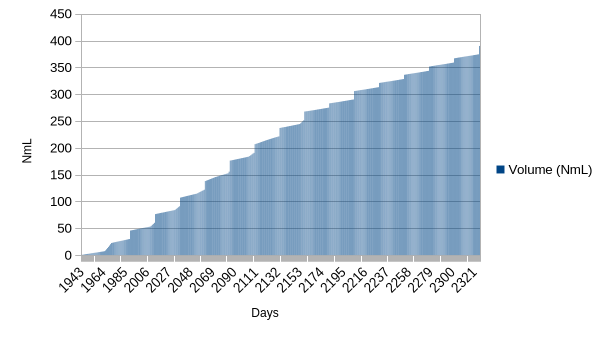
\includegraphics[width=\textwidth]{assets/graphs/extra-accumulation.png}
    \caption{Source: Author}
    \label{graph:extra-accumulation}
\end{graph}

\begin{graph}
    \centering
    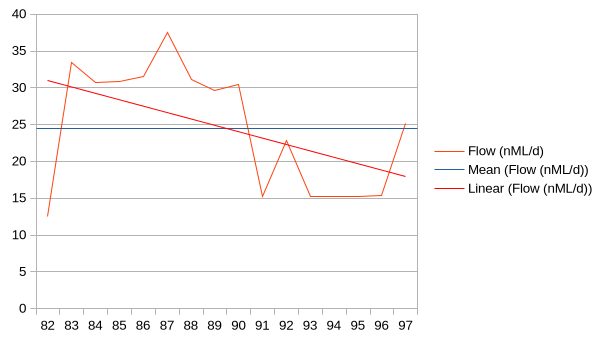
\includegraphics[width=\textwidth]{assets/graphs/extra-flow.png}
    \caption{Source: Author}
    \label{graph:extra-flow}
\end{graph}

\subsection{Alkalinity and Volatile Fatty Acids}
\label{subsec:alkalinity_vfa}

The total alkalinity and VFA concentrations were monitored throughout the experiment to assess process stability. The results are shown in \cref{graph:alkalinity_vfa}. Initially, both alkalinity and VFA were low, reflecting the early adaptation phase before buffer addition. After the manual introduction of KHCO$_3$, alkalinity increased sharply to values above 7000 mg CaCO$_3$/L and remained relatively high until close to the end. This high alkalinity was maintained by the addition of bicarbonate to the feed, which helped to counteract the acidity produced during the degradation of the feed.

VFA concentrations also increased after the start of feeding, reaching values between 3000 and 5000 mg CH$_3$COOH/L. Such high VFA levels are often associated with process imbalance, as they can inhibit methanogenesis. However, the high alkalinity provided a strong buffering capacity, and the pH remained above 6.5 for most of the experiment, with the co-digestion the pH was falling and with glycerol only the pH was increasing. The VFA/alkalinity ratio is a more reliable indicator of instability. In this experiment, the ratio fluctuated between 0.3 and 1.2. While using the co-digestion feed a ration aroun 0.8 to 1.0 had the highest production.

\begin{graph}
    \centering
    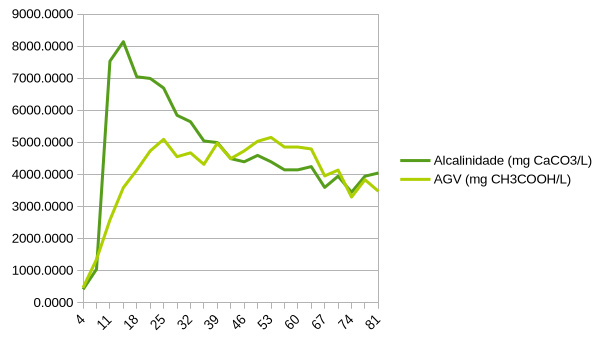
\includegraphics[width=\textwidth]{assets/graphs/alcalinidade-agv.png}
    \caption{Source: Author}
    \label{graph:alkalinity_vfa}
\end{graph}

\begin{graph}
    \centering
    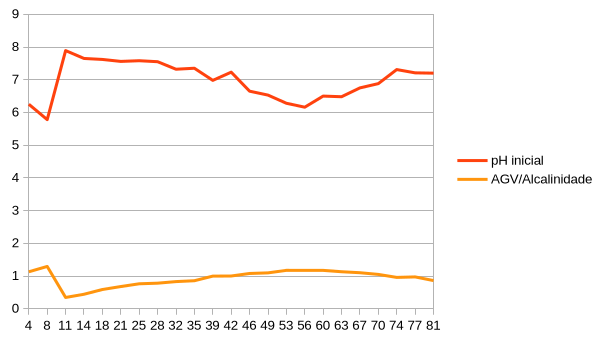
\includegraphics[width=\textwidth]{assets/graphs/ph-razao.png}
    \caption{Source: Author}
    \label{graph:ph_ratio}
\end{graph}

\subsection{Subestrate used as feed}
\label{subsec:sub_feed}

\Cref{tab:feeds} shows all substrates used to feed the reactor and when they were made.

\begin{footnotesize}
    \begin{ThreePartTable}
        \begin{xltabular}{\linewidth}{@{} C C C C C C C @{}}

        \caption{Source:Author}
        \label{tab:feeds} \\

        \toprule
        \thead{Day} &
        \thead{Substrate 1} &
        \thead{Subestrate 2} &
        \thead{Substrate 3} &
        \thead{Extra\\ Addition} &
        \thead{COV\\ \& TS\%} &
        \thead{Volume\\ Made} \\
        \midrule
        \endfirsthead

        \multicolumn{6}{l}{\textit{\Cref{tab:feeds} continued}} \\
        \toprule
        \thead{Day} &
        \thead{Substrate 1} &
        \thead{Subestrate 2} &
        \thead{Substrate 3} &
        \thead{Extra\\ Addition} &
        \thead{COV\\ \& TS\%} &
        \thead{Volume\\ Made} \\
        \midrule
        \endhead

        \bottomrule
        \endlastfoot

        0\tnote{a} &
        Food Waste, 156 g &
        Glucose, 1.9 g &
        &
        Calcium Bicarbonate, 5 g &
        1.5 \& 15 &
        500 mL\\
        \addlinespace
        4 &
        Crude Glicerol, \approx 23.2 mL &
        Pure Glicerol\tnote{b}, \approx 31.5 mL &
        &
        Potassium Bicarbonate, \approx 1.9 g &
        0.8 \& 10 &
        250 mL\\
        \addlinespace
        11 &
        Food Waste, \approx 12.54 g &
        Crude Glicerol, \approx 9.02 mL &
        Pure Glicerol, \approx 2.6 mL &
        Potassium Bicarbonate, \approx 1.57 g &
        0.13-0.4 \& 5-10 &
        250 mL\\
        \addlinespace
        18 &
        Food Waste, \approx 10.88 g &
        Crude Glicerol, \approx 2.89 mL &
        Pure Glicerol, \approx 1.44 mL &
        &
        0.0256 \& \approx 2 &
        250 mL\\
        \addlinespace
        25 &
        Food Waste, \approx 31.12 g &
        Crude Glicerol, \approx 44 mL &
        Pure Glicerol, \approx 29 mL &
        &
        \approx 1.4 \& \approx 10 &
        250 mL \\
        \addlinespace
        32 &
        Food Waste, \approx 31.01 g &
        Crude Glicerol, \approx 44 mL &
        Pure Glicerol, \approx 28.9 mL &
        &
        \approx 1.4 \& \approx 10 &
        250 mL \\
        \addlinespace
        39 &
        Food Waste, \approx 46.52 g &
        Crude Glicerol, \approx 66 mL &
        Pure Glicerol, \approx 43 mL &
        Potassium Bicarbonate, \approx 2.6 g &
        \approx 3.1 \& \approx 15 &
        250 mL \\
        \addlinespace
        46 &
        Food Waste, \approx 50.07 g &
        Crude Glicerol, \approx 66 mL &
        Pure Glicerol, 43 mL &
        Potassium Bicarbonate, \approx 2.67 g &
        \approx 3.16 \& \approx 15 &
        250 mL \\
        \addlinespace
        53\tnote{c} &
        Crude Glicerol, \approx 55 mL &
        Pure Glicerol, \approx 11.5 mL &
        &
        Potassium Bicarbonate, \approx 5.38 g &
        0.42 \& \approx 10 &
        500 mL \\
        \addlinespace
        60 &
        Crude Glicerol, \approx 55 mL &
        Pure Glicerol, \approx 12 mL &
        &
        Potassium Bicarbonate, \approx 5.18 g &
        0.42 \& \approx 10 &
        500 mL\tnote{d} \\
        \addlinespace
        67 &
        Crude Glicerol, \approx 41 mL &
        Pure Glicerol, \approx 9 mL &
        &
        Potassium Bicarbonate, \approx 2.56 g &
        0.95 \& \approx 15 &
        250 mL \\
        \addlinespace
        74 &
        Crude Glicerol, \approx 60 mL &
        Pure Glicerol, \approx 12.5 mL &
        &
        Potassium Bicarbonate, \approx 2.57 g &
        \approx 1.37 \& \approx 15 &
        250 mL \\

        \end{xltabular}

        \begin{tablenotes}
            \item[a] It only started feeding on day 2.
            \item[b] The solution of pure glicerol was diluted 100X.
            \item[c] Change of substrate.
            \item[d] There was a leak on the feeding tube.
        \end{tablenotes}
    \end{ThreePartTable}
\end{footnotesize}
